\begin{solution}
\begin{enumerate}
\item {[3 points]} The definition of $\phi_j$ yields that $\phi_j(x_k)=0$ if $k\ne j$. Moreover,
\[\phi_j(x_j)=\frac{x_{j+1}-x_j}{h}=\frac{(j+1)h-jh}{h}=\frac{jh+h-jh}{h}=\frac{h}{h}=1.\]
Consequently, for $j=1,\ldots,N$,
\[ \phi_j(x_k) = \left\{ \begin{array}{l}
1\mbox{ if }k=j, \\
0\mbox{ if }k\ne j,
\end{array}\right. \]
for $k=0,1,\ldots,N+1$.
\\
\item {[3 points]} If $c_k\in\mathbb{R}$ and $\displaystyle{\sum_{k=1}^N}c_k\phi_k(x)=0$ for all $x\in[0,1]$ then $\displaystyle{\sum_{k=1}^N}c_k\phi_k(x_j)=0$ for $j=1,\ldots,N$. The answer to part (a) then allows us to conclude that $c_j=0$ for $j=1,\ldots,N$ since $\displaystyle{\sum_{k=1}^N}c_k\phi_k(x_j)=c_j$. Therefore, $c_k=0$ for $k=1,\ldots,N$ since $c_j=0$ for $j=1,\ldots,N$ is equivalent to $c_k=0$ for $k=1,\ldots,N$.
\\
\item {[3 points]} For $j=1,\ldots,N$, integrating by parts yields that
          \begin{eqnarray*}
\int_{x_{j-1}}^{x_j} {x-x_{j-1} \over h} \sin(\pi x)\, dx&=&\left[{x-x_{j-1} \over h}\left(-{\cos(\pi x) \over \pi}\right)\right]_{x_{j-1}}^{x_j}+\int_{x_{j-1}}^{x_j}\frac{d}{dx}\left({x-x_{j-1} \over h}\right) {\cos(\pi x) \over \pi}\, dx \\[0.5em]
&=&-{x_j-x_{j-1} \over h}{\cos(\pi x_j) \over \pi}+\int_{x_{j-1}}^{x_j}{1 \over h}{\cos(\pi x) \over \pi}\, dx\\[0.5em]
&=&-{jh-(j-1)h \over h}{\cos(\pi x_j) \over \pi}+\left[{1 \over h}{\sin(\pi x) \over \pi^2}\right]_{x_{j-1}}^{x_j}\\[0.5em]
&=&-{\cos(\pi x_j) \over \pi}+{\sin(\pi x_j)-\sin(\pi x_{j-1}) \over \pi^2h}
         \end{eqnarray*} 
and
          \begin{eqnarray*}
\int_{x_j}^{x_{j+1}} {x_{j+1}-x \over h} \sin(\pi x)\, dx&=&\left[{x_{j+1}-x \over h}\left(-{\cos(\pi x) \over \pi}\right)\right]_{x_j}^{x_{j+1}}+\int_{x_j}^{x_{j+1}}\frac{d}{dx}\left({x_{j+1}-x \over h}\right) {\cos(\pi x) \over \pi}\, dx \\[0.5em]
&=&{x_{j+1}-x_j \over h}{\cos(\pi x_j) \over \pi}-\int_{x_j}^{x_{j+1}}{1 \over h}{\cos(\pi x) \over \pi}\, dx\\[0.5em]
&=&{(j+1)h-jh \over h}{\cos(\pi x_j) \over \pi}-\left[{1 \over h}{\sin(\pi x) \over \pi^2}\right]_{x_j}^{x_{j+1}}\\[0.5em]
&=&{\cos(\pi x_j) \over \pi}+{\sin(\pi x_j)-\sin(\pi x_{j+1}) \over \pi^2h}.
         \end{eqnarray*} 
Hence, for $j=1,\ldots,N$,
          \begin{eqnarray*}
              \ip{f,\phi_j} &=& \int_{x_{j-1}}^{x_j} {x-x_{j-1} \over h} \sin(\pi x)\, dx
                              + \int_{x_j}^{x_{j+1}} {x_{j+1}-x \over h} \sin(\pi x)\, dx \\[0.5em]
                             &=& {2 \sin(\pi x_j) - \sin(\pi x_{j-1}) - \sin(\pi x_{j+1}) 
                                   \over \pi^2 h} \\[0.5em]
                             &=& {2\sin(\pi x_j) \over \pi^2 h} (1 - \cos(h\pi)).
         \end{eqnarray*} 
\\
\item {[8 points]} For $j=1,\ldots,N$, letting $s=x-x_{j-1}$ and $t=x-x_{j+1}$ yields that
\begin{eqnarray*}
\ip{\phi_j, \phi_j} &=& \int_0^1\left(\phi_j(x)\right)^2\, dx
\\
&=& \int_0^{x_{j-1}}\left(\phi_j(x)\right)^2\, dx+\int_{x_{j-1}}^{x_j}\left(\phi_j(x)\right)^2\, dx+\int_{x_j}^{x_{j+1}}\left(\phi_j(x)\right)^2\, dx+\int_{x_{j+1}}^1\left(\phi_j(x)\right)^2\, dx
\\
&=& \int_0^{x_{j-1}}0\, dx+\int_{x_{j-1}}^{x_j} \left({x-x_{j-1} \over h}\right)^2\, dx + \int_{x_j}^{x_{j+1}} \left({x_{j+1}-x \over h}\right)^2\, dx+\int_{x_{j+1}}^10\, dx
\\
&=& \int_{x_{j-1}}^{x_j} \left({x-x_{j-1} \over h}\right)^2\, dx + \int_{x_j}^{x_{j+1}} \left({x_{j+1}-x \over h}\right)^2\, dx
\\
&=& {1\over h^2}\int_{x_{j-1}-x_{j-1}}^{x_j-x_{j-1}} \left(s+x_{j-1}-x_{j-1}\right)^2\, ds + {1\over h^2}\int_{x_j-x_{j+1}}^{x_{j+1}-x_{j+1}} \left(x_{j+1}-\left(t+x_{j+1}\right)\right)^2\, dt
\\
&=& {1\over h^2}\int_0^h s^2\, ds + {1\over h^2}\int_{-h}^0 t^2\, dt
\\
&=& {1\over h^2}\left[ {s^3 \over 3}\right]_0^h+{1\over h^2}\left[ {t^3 \over 3}\right]_{-h}^0
\\
&=& {h^3 \over 3h^2} - {(-h)^3 \over 3h^2}
\\
&=& {h \over 3} + {h \over 3}
\\
&=& {2h\over 3}.
\end{eqnarray*}

Moreover, for $j=1,\ldots,N-1$,
\[
\phi_{j+1}(x) = \left\{
\begin{array}{ll}
\displaystyle{{x-x_j\over h}} & \mbox{if }x\in [x_j, x_{j+1});\\
\displaystyle{{x_{j+2}-x\over h}} & \mbox{if }x\in [x_{j+1}, x_{j+2});\\
0 & \mbox{otherwise};
\end{array}\right.
\]
and so letting $s=x-x_j$ yields that
\begin{eqnarray*}
\ip{\phi_{j+1}, \phi_j} &=& \ip{\phi_j, \phi_{j+1}}
\\
 &=& \int_0^1\phi_j(x)\phi_{j+1}(x)\, dx
\\
&=& \int_0^{x_j}\phi_j(x)\phi_{j+1}(x)\, dx+\int_{x_j}^{x_{j+1}}\phi_j(x)\phi_{j+1}(x)\, dx+\int_{x_{j+1}}^1\phi_j(x)\phi_{j+1}(x)\, dx
\\
&=& \int_0^{x_j}0\, dx+ \int_{x_j}^{x_{j+1}} {x_{j+1}-x \over h}{x-x_j\over h}\, dx+\int_{x_{j+1}}^10\, dx
\\
&=& \int_{x_j}^{x_{j+1}} {x_{j+1}-x \over h}{x-x_j\over h}\, dx
\\
&=&  {1\over h^2}\int_{x_j-x_j}^{x_{j+1}-x_j} \left(x_{j+1}-(s+x_j)\right)\left(s+x_j-x_j\right)\, ds
\\
&=&  {1\over h^2}\int_{0}^{h} hs-s^2\, ds
\\
&=&  {1\over h^2}\left[{hs^2\over 2}-{s^3\over 3}\right]_0^h
\\
&=&  {1\over h^2}\left({h^3\over 2}-{h^3\over 3}\right)
\\
&=&  {3\over 6}-{2h\over 6}
\\
&=& {h\over 6}.
\end{eqnarray*}

Finally, for $j=1,\ldots,N$,
\[
\ip{\phi_j, \phi_k}=\int_0^1\phi_j(x)\phi_k(x)\, dx=\int_0^10\, dx=0
\]
if $\left|j-k\right|>1$.

Hence, for $j,k=1,\ldots,N$,
\[
\ip{\phi_j,\phi_k}=\left\{\begin{array}{ll}{2h \over 3} & \mbox{if }k=j, \\[.75em] {h \over 6} & \mbox{if }\left|j-k\right|=1, \\[.75em] 0 & \mbox{otherwise}.\end{array}\right.
\]
\\
\item {[8 points]} The requested plots are shown below, followed by the MATLAB code that generated them.

\begin{center}
   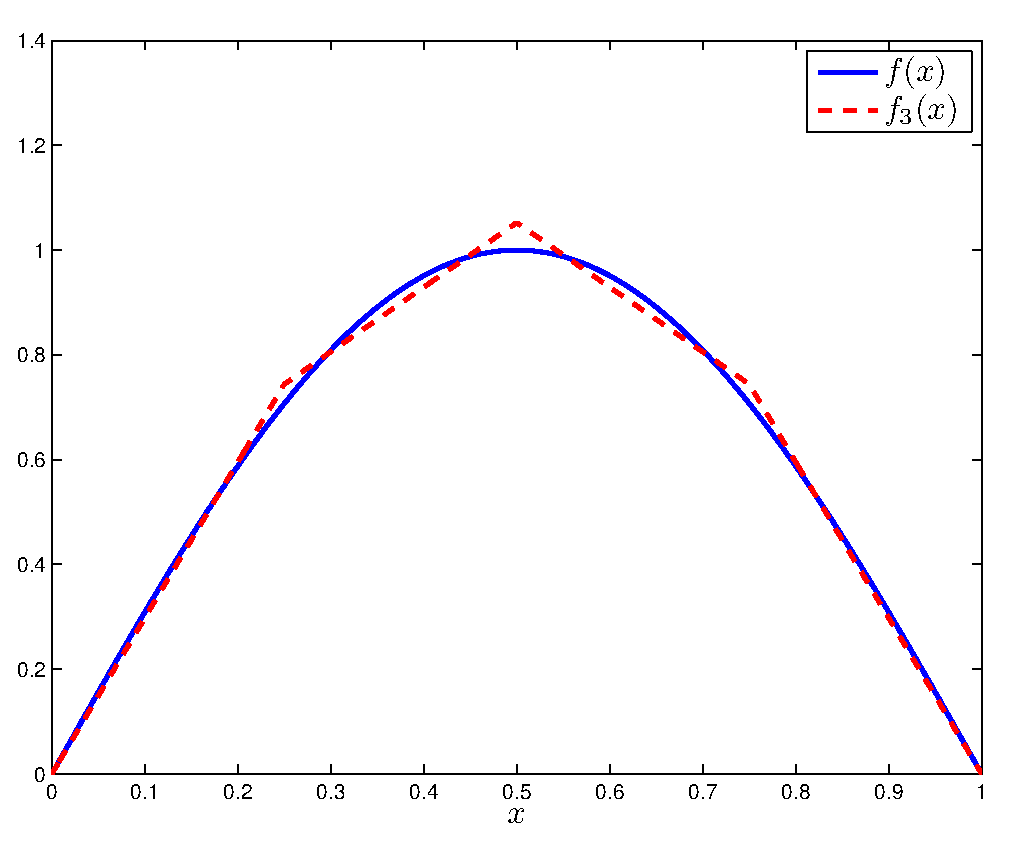
\includegraphics[scale=0.4]{f_3}
   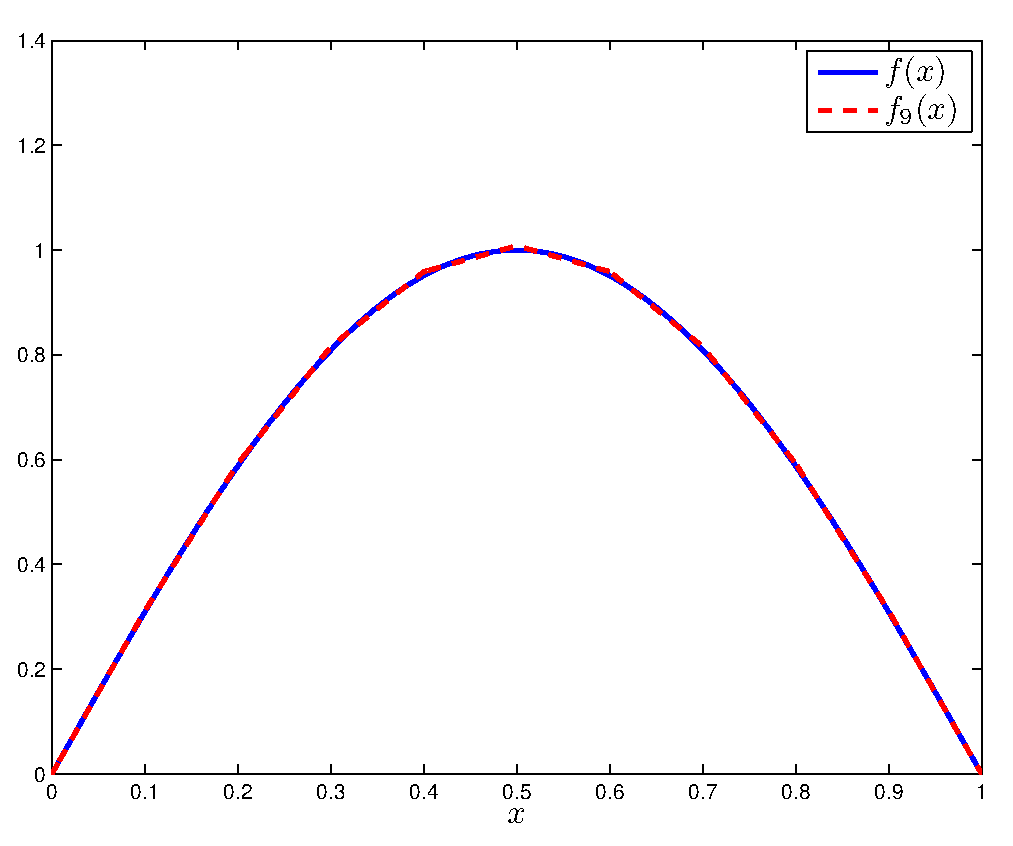
\includegraphics[scale=0.4]{f_9}
\end{center}

\lstinputlisting{HW15e.m}
\end{enumerate}
\end{solution}